\section{Experiments}
I performed experiments to evaluate the performances of similarity measures and algorithms in Section~\ref{sec:connectionsimilarity}.
\newline
In Section~\ref{subsec:datasetandsetup}, I describe the dataset that I used for the experiements.\newline
In Section~\ref{subsec:detectinganomalies}, I evaluate how successful the algorithms are in detecting different types of anomalies.

\subsection{Dataset and Setup}
\label{subsec:datasetandsetup}
KDD 99 dataset is mainly used for network-based intrusion detection algorithm evaluation\cite{tavallaee09}. 
Specifically I select the NSL-KDD dataset which is an up-to-date version of KDD dataset. 
Since the NSL-KDD dataset solves issues in the original data set, I use the data set in this report as an effective benchmark. 
Also its relevance of each feature in the data set is also studied\cite{olusola10} \cite{kayacik05}. 
% All source code is on the Internet. 
% I use NSL-KDD99 Dataset for the report. 
% semi-supervised approach

\begin{figure}[htb2]
\begin{center}
%\begin{inparaenum}[\itshape a\upshape)]
%\item data preprocessing
%\item data transformation
%\item affinity matrix computation
%\item clustering
%\item outlier detection
%\end{inparaenum}
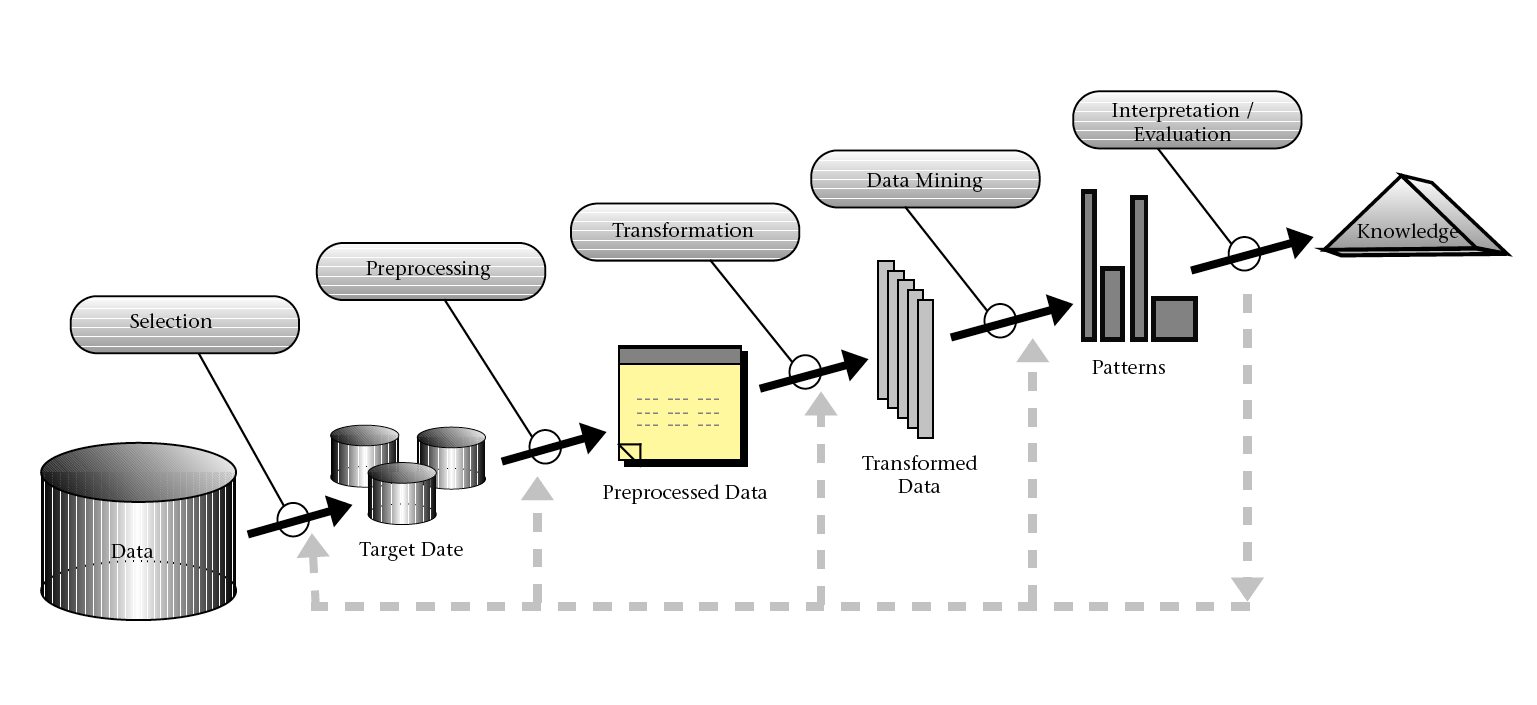
\includegraphics[width=5.5in,angle=0]{./sections/Fayyad96kdd-process.eps}
\end{center}
\caption{Overview of Intrusion Detection System}
\label{fig:refSingleRobot1}
\end{figure}
The intrusion detection system should find specific kinds of abnomal traffic e.g. a denial of service (DoS) attack. 
It should check if these new sets of mornitoring data show similar properties as the orignal data or not as well. 
I construct the system similar to knowledge discovery system \cite{fayyad96} because it is widely used among intrusion detection systems. 
A new approach to construct a pairwise similarity matrix is that compares their probability in pairwise not its attributes directly. 
For this, the system includes gaussian mixture models (GMM) for attributes and classes to calculate the probability for data point.
The EM approach is used to fit those models and is guaranteed to converge to a local optimum on given input. 
With those components, we measure a score for each attributes, and those scores are weighted based on their importance in the dataset\cite{kayacik05}.
%to get 2D data where x-axis is a score for normal connection similarity and y-axis is a score for known abnormal connection similarity. 
The experiment suggest that such local optimum can effectively seperate different connections and most of unknown classes. 
\begin{figure}[htb2]
\begin{center}
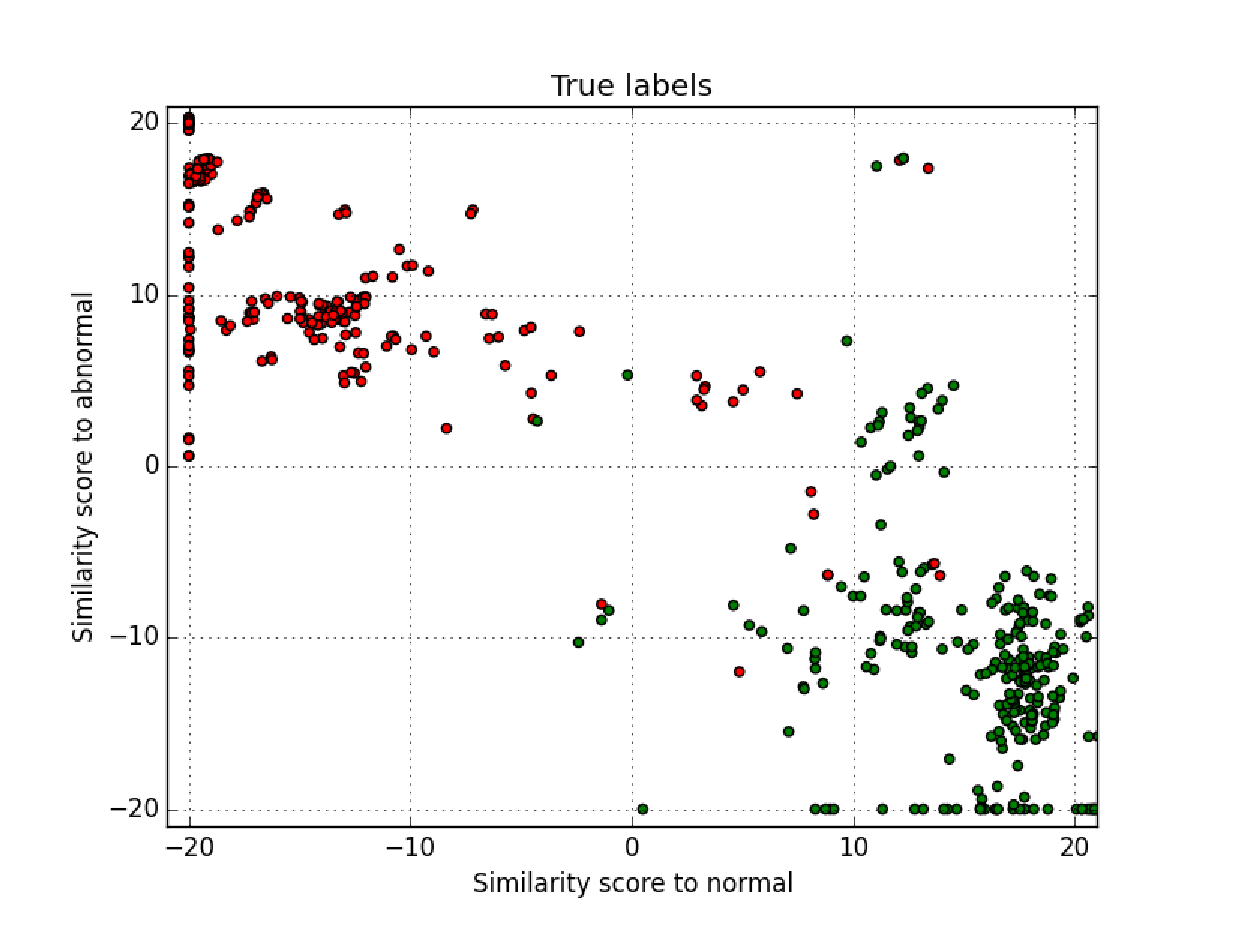
\includegraphics[width=3.5in,angle=0]{./sections/training20_only_true_.eps}
\end{center}
\caption{Similarity of normal and abnormal connections in training set.}
% The left figure shows data points including known anomalies and the right known type of anomalies shows data points including unknown type of anomalies.} % I may show rest of data in appendix
\label{fig:refSingleRobot1}
\end{figure}

%In order for spectral anaysis, we need to make a sparse affinity matrix from transported data. 
%We can compute a sparse affinity matrix from a pairwise similarity matrix. 
After we have a pairwise similarity matrix, one way to convert similarity matrix to a sparse affinity matrix is that dealing with the affinities for $k$ nearest neighborhood only, and set all other values for current data point to zero. 
I choose the $k = 8$ because it is commonly used in spectral clustering. 

% Altho require non-convex boundaries,
%\subsection{Computing affinity matrix}
%%The processing steps of the approach can be summerized as follows:
%%1) Training mixture model with training set containing records of both normal and anomalous connections.
%%2) The data are divided into different clusters for normal and anomalous connections using Spectral clustering algorithm.
%\subsubsection{Data pre-processing}
%\begin{itemize}
%\item categorical value to integer e.g.) service-type (ftp-data,http,etc).
%\item log of big number e.g.) duration, src-bytes.
%\end{itemize}
%\subsubsection{Affinity matrix computation}
%The data points are associated with each other by pairwise similarity.
%\begin{itemize}
%\item Construct similarity matrix with distance metric.
%\item Construct affinity matrix from similarity matrix with 8-nearest neighbors algorithm.
%\end{itemize}
%\subsection{Clustering}
%%\subsubsection{Number of clusters prediction}
%%Predict number of clusters based on the eigengap.
%%\subsubsection{Spectral clustering algorithm}
%%Normalized cut algorithm. \cite{jianbo00}
%%\subsubsection{Representative of clusters}
%%Clusters are represented by the mean and variance.
%\subsection{Detecting anomaly from clusters}
%%Distance based outlier detection is used.
%%\begin{itemize}
%%\item It do not require any prior knowledge.
%%\item k-nearest neighbor outlier detection algorithm. \cite{knorr00}
%%\end{itemize}

\subsection{Detecting Anomalies}
\label{subsec:detectinganomalies}
In this section, I describe how the a sparse affinity matrix can be used to detect point and collective anomalies. 
In the following experiments, I divide experiments for known anomalies and unknown anomalies. 

\subsubsection{Known Anomalies}
We see that normal and abnormal connections similarity are sensitive to known anomalies. 
It shows how similarity measure captures the effect of an known anomaly. 
% The similarity coputed by mixture models gives similarity scores that are used to find k nearest neighborhood.

\begin{figure}[htb2]
\begin{center}
\subfloat[Predicted labels]{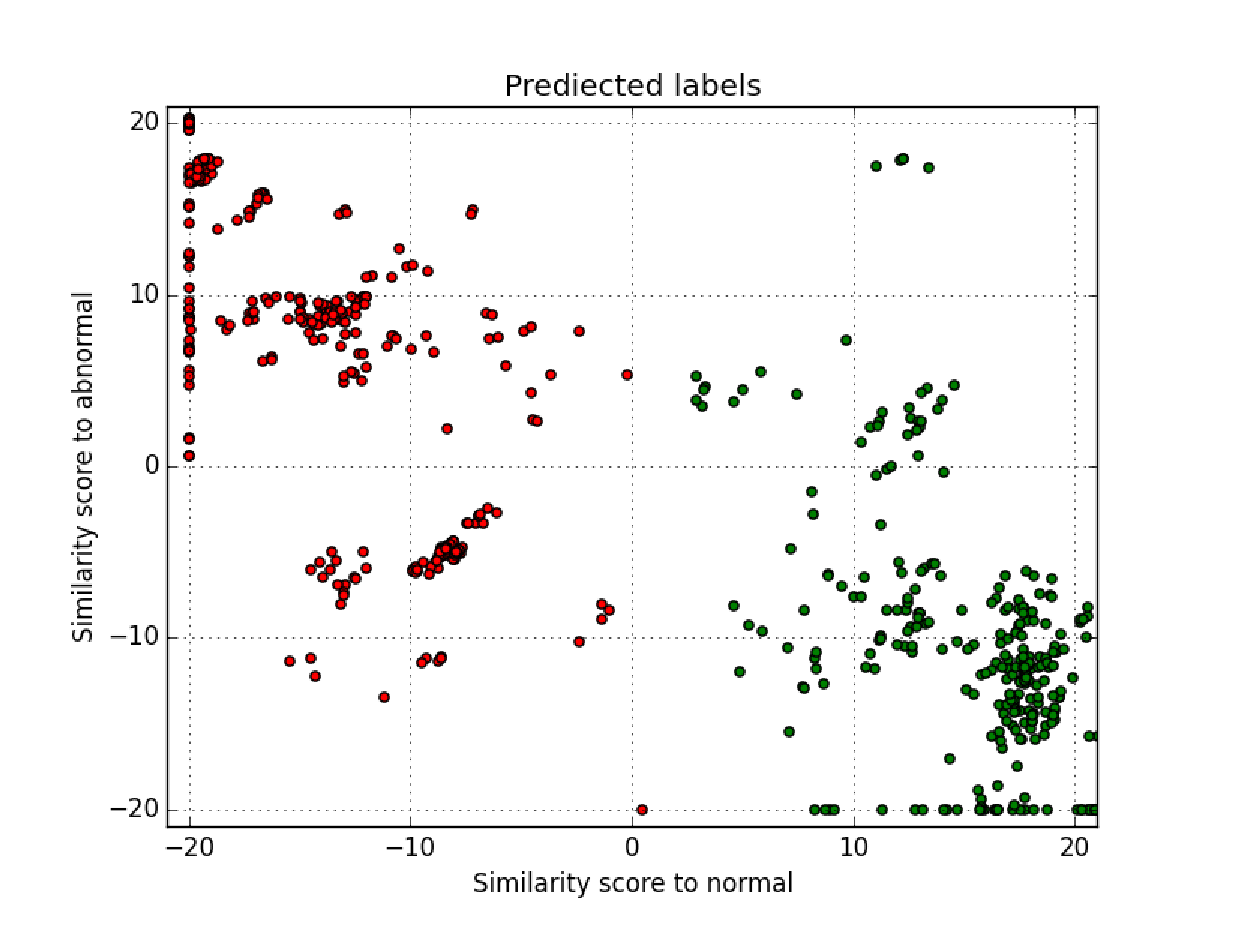
\includegraphics[width=3.5in,angle=0]{./sections/training20_test20_back_prediction_.eps}}
\subfloat[True labels]{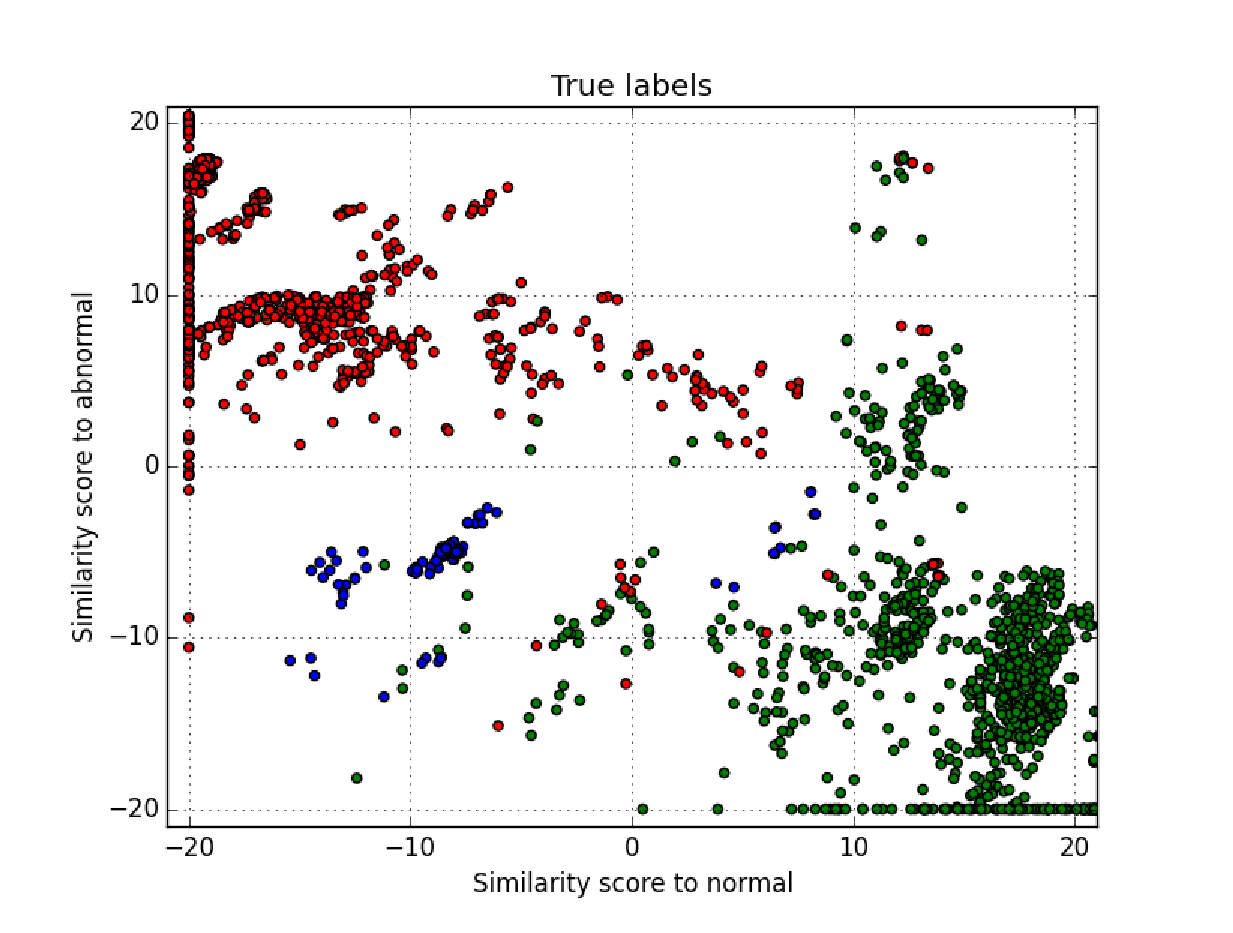
\includegraphics[width=3.5in,angle=0]{./sections/training20_test20_back_true_.eps}}
\end{center}
\caption{Similarity of normal and abnormal connections in training set} % I may show rest of data in appendix
\label{fig:refSingleRobot1}
\end{figure}
%Result provides the sensitivity and the coverage of similarity measure that is effective. 
%All data point in testset for 21 known abnomal classes shows similar to known anomalies. 
%After it calcurate the similarity among data points 
For all class, the similarity is very close either normal or abnormal connections. 
\begin{table}[h]
\begin{center}
\begin{tabular}{| l | l | l | p{5cm} |}
\hline
Type of Anomaly & Predicted normal & Predicted anormalies & $\%$ correct\\
\hline
True normal &  &  & \\
\hline
True anormalies &  &  & \\
\hline
\end{tabular}
\end{center}
\caption{Abnomal classes in NSL-KDD99}
\label{fig:refSingleRobot1}
\end{table}

In summary, all the class successfully detect known anomalies in spectral approach. 
% The detection rate for them are quite high. 

\begin{figure}[htb2]
\begin{center}
\end{center}
\caption{Clusters of connections including known anomalies. The x-axis shows the normal similarity scores and the y-axis shows the known abnormal similarity scores}
\label{fig:refSingleRobot1}
\end{figure}

\subsubsection{Unknown Anomalies}
We see that normal and abnormal connection similarity are also sensitive to most of unknown anomaly. 
However, we have four classes that is similar to normal connections. 
Connection density similarity measure is sensitive in this type of anomaly if it is above its threshold. 
However this approach does not work if the data points are insufficient to form high density.

Here 4 out of 17 are close to known normal connections. 
We can detect them with exactly same way what it have done to known anomalies since their performance is also good. 
\begin{table}[h]
\begin{center}
\begin{tabular}{| l | l | l | p{5cm} |}
\hline
Type of Anomaly & Predicted normal & Predicted anormalies & $\%$ correct\\
\hline
True normal &  &  & \\
\hline
True anormalies (close to A)&  &  & \\
\hline
True anormalies (close to N) &  &  & \\
\hline
\end{tabular}
\end{center}
\caption{Abnomal classes in NSL-KDD99}
\label{fig:refSingleRobot1}
\end{table}

13 out of 17 unknown and unseen anomalies are similar to known and seen anomalies such as processtable class. 
However 4 out of 17 are close to normal connections in training set. 
In that case, a cluster resulted by spectral clustering shows abnomal density if we compare with a cluster formed by normal connections only. 
So with those prior knowledge we can use spectral approach to find abnormal clusters which is originally classified as normal connection. 
However we can not detect anomalies which are too few to form enough density such as snmpguess or snmpgetattack class. 
\begin{figure}[htb2]
\begin{center}
\subfloat[Predicted labels]{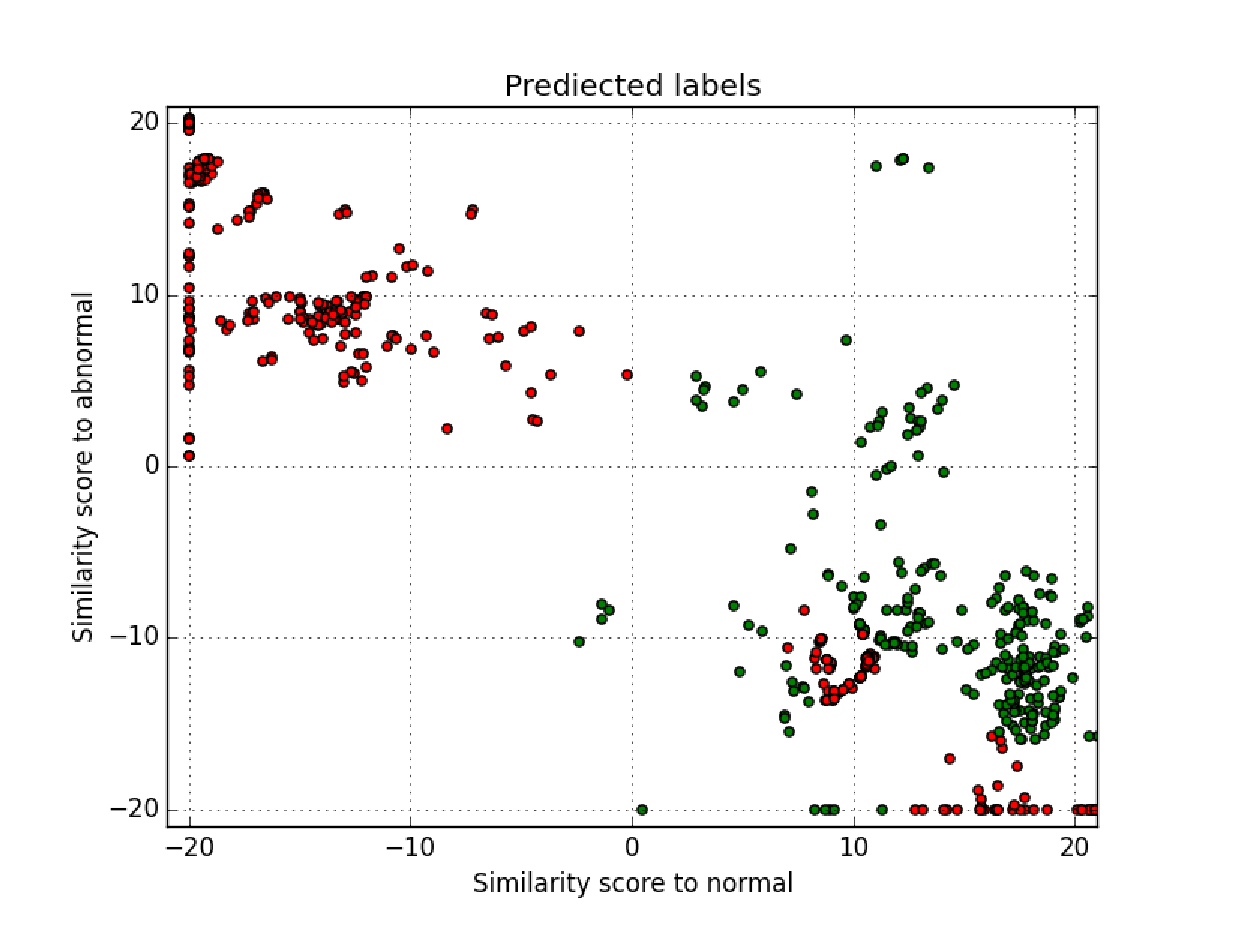
\includegraphics[width=3.5in,angle=0]{./sections/training20_test20_mailbomb_prediction_.eps}}
\subfloat[True labels]{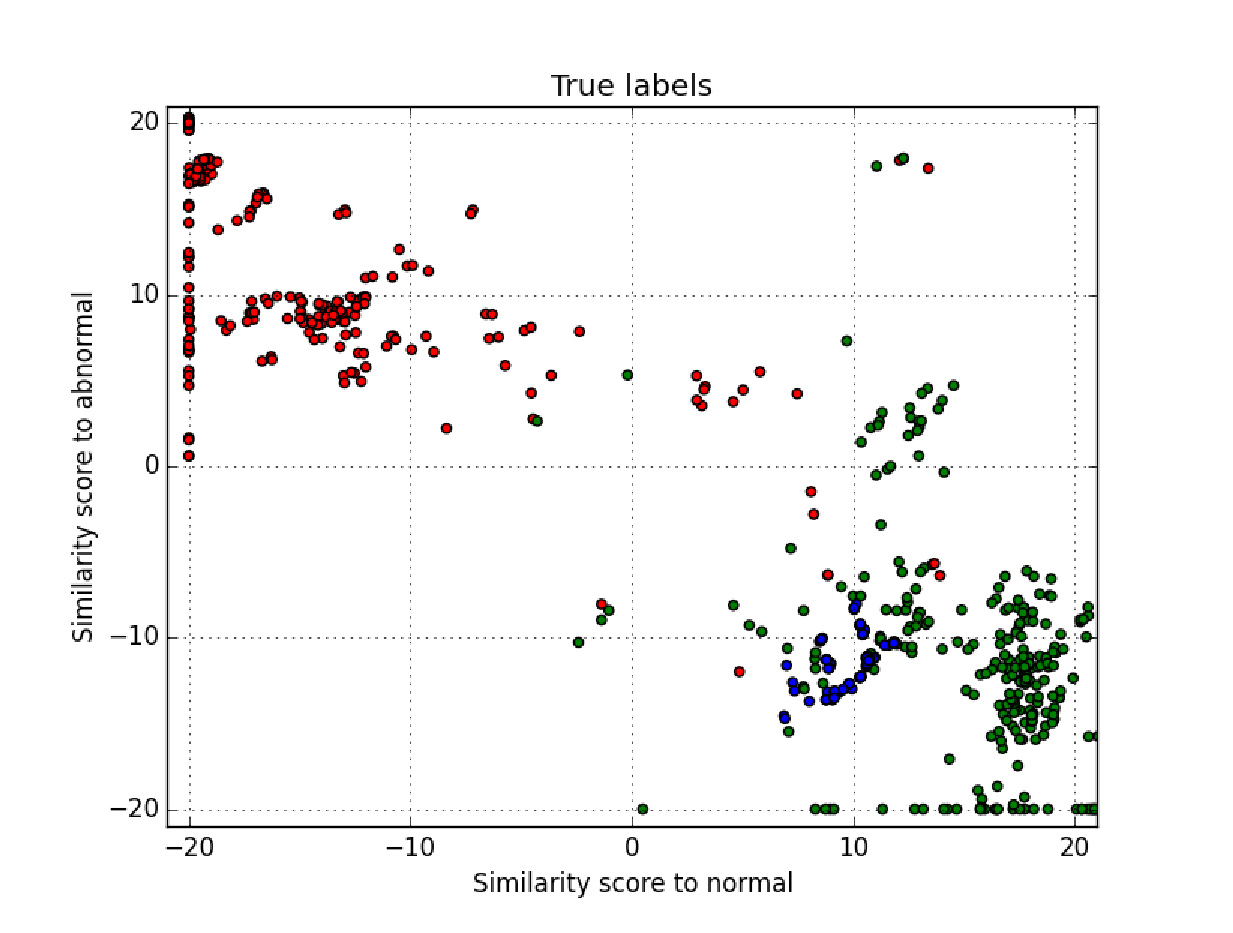
\includegraphics[width=3.5in,angle=0]{./sections/training20_test20_mailbomb_true_.eps}}
\end{center}
\caption{Density based intrusion detection result for unknown anomalies.} % I may show rest of data in appendix
\label{fig:refSingleRobot1}
\end{figure}


